\documentclass[titlepage]{jsarticle}
\usepackage[dvipdfmx]{graphicx}
\usepackage{here}
\usepackage{bm}
\usepackage{amsmath}
\usepackage{amssymb}
\usepackage{amsfonts}
\usepackage{comment}
\usepackage{listings}
\lstset{
    basicstyle={\ttfamily},
    identifierstyle={\small},
    commentstyle={\smallitshape},
    keywordstyle={\small\bfseries},
    ndkeywordstyle={\small},
    stringstyle={\small\ttfamily},
    frame={tb},
    breaklines=true,
    columns=[l]{fullflexible},
    numbers=left,
    xrightmargin=0zw,
    xleftmargin=3zw,
    numberstyle={\scriptsize},
    stepnumber=1,
    numbersep=1zw,
    lineskip=-0.5ex,
    keepspaces=true,
    language=c
}
\renewcommand{\lstlistingname}{ソースコード}
\makeatletter
\newcommand{\figcaption}[1]{\def\@captype{figure}\caption{#1}}
\newcommand{\tblcaption}[1]{\def\@captype{table}\caption{#1}}
\makeatother




\begin{document}
\title{数値解析レポートNo.4}
\author{37番 本間三暉}
\date{}
\maketitle

\section{連立微分方程式}
以下を満たす$(x,y)$を$t=[0,2]$の範囲で求める。
\begin{eqnarray}
	\frac{dx}{dt} &=& x + 6y -10,\; \; x(0) = 1\nonumber \\
	\frac{dy}{dt} &=& x + t -3, \;\; y(0) = 2 \nonumber
\end{eqnarray}

$\dfrac{dx}{dt} = f(x,y;t),\dfrac{dy}{dt} = g(x,y;t)$と考える。積分区間を分割した時の$x_{i+1},y_{i+1}$は
\begin{eqnarray}
	x_{i+1} = x_i + f(x_i,y_i;t_i) * \Delta t \nonumber \\
	y_{i+1} = y_0 + g(x_i,y_i;t_i) * \Delta t \nonumber
\end{eqnarray}
と考えることができる。これを利用し
連立微分方程式の解を求めるプログラムをソースコード\ref{src:1}に示す。

\begin{lstlisting}[caption=作成した連立微分方程式を解くプログラム, label=src:1]
double f(double x, double y, double t) {
	return x + 6 * y + t - 10;
}
double g(double x, double y, double t) {
	return x + t - 3;
}
double true_x(double t) {
	return -2 * exp(-2 * t) - t + 3;
}
double true_y(double t) {
	return exp(-2 * t) + 1;
}
int main()
{
	double x[N], y[N];
	double l = 0, r = 2, t = 0;
	int n;
	double dt = (l + r) / N;
	int i;

	x[0] = 1;
	y[0] = 2;

	printf("%.6lf, %.6lf, %.6lf, %.6lf, %.6lf\n", 
		t, x[0], y[0], true_x(t), true_y(t));
	for (i = 1; i <= N; i++) {
		t += dt;
		x[i] = x[i - 1] + f(x[i - 1], y[i - 1], t) * dt;
		y[i] = y[i - 1] + g(x[i - 1], y[i - 1], t) * dt;
		printf("%.6lf, %.6lf, %.6lf, %.6lf, %.6lf\n", 
			t, x[i], y[i], true_x(t), true_y(t));
	}
}
\end{lstlisting}
このプログラムによって、求めた$x(t),y(t)$と真の$x(t),y(t)$とを比較した様子を、それぞれ図\ref{fig:x(t)},\ref{fig:y(t)}に示す。
どちらもNは分割数を示している。これらの図を見ると、ステップ幅を小さくすればするほど真の解に近づいていくことがわかる。
\begin{figure}[H]
	\centering
	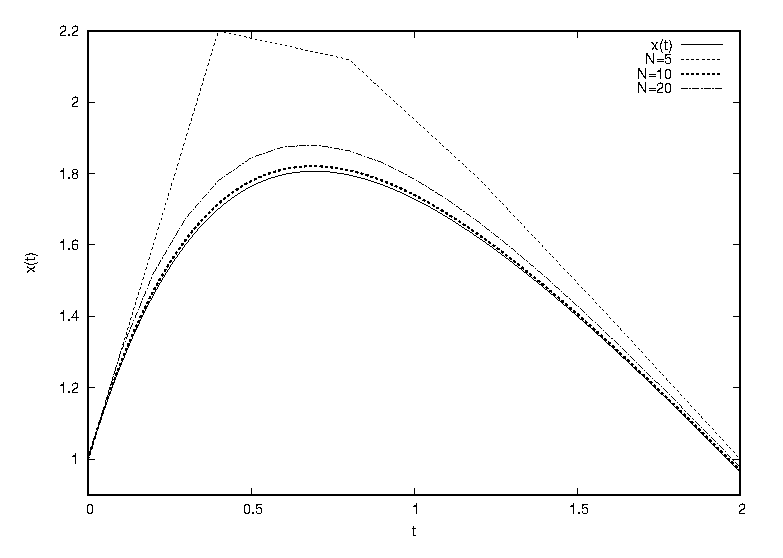
\includegraphics[height=7cm]{1/x(t).eps}
	\caption{真のx(t)と求めたx(t)との比較}
	\label{fig:x(t)}
\end{figure}
\begin{figure}[H]
	\centering
	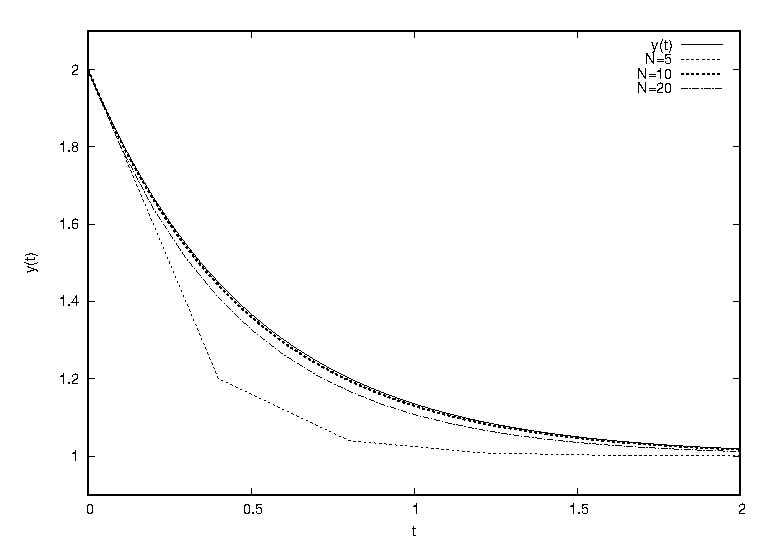
\includegraphics[height=7cm]{1/y(t).eps}
	\caption{真のy(t)と求めたy(t)との比較}
	\label{fig:y(t)}
\end{figure}

%ホイン方とかやる?

\section{高次微分方程式}
$x=1$における以下の微分方程式の解$y$を求める。
\begin{eqnarray}
	\frac{d^2y}{dx^2}+5\frac{dy}{dx}-6y = 0 \label{equ:2} \\
	\;\; y(0) = 0,\;\;\frac{dy}{dx}(0)=7 \nonumber
\end{eqnarray}
$\dfrac{dy}{dx} = z$とおくと$\dfrac{d^2y}{dx^2} = \dfrac{dz}{dx}$となるので、これを式(\ref{equ:2})に代入すると
以下のような連立微分方程式となる。
\begin{eqnarray}
	\frac{dy}{dx} &=& z \nonumber \\
	\frac{dz}{dx} &=&  6y -5z \nonumber
\end{eqnarray}
これは前章と同じように解くことができる。前章のように$x=[0,2]$の範囲で$y(x)$グラフを描くと以下のようになる。
\begin{figure}[H]
	\centering
	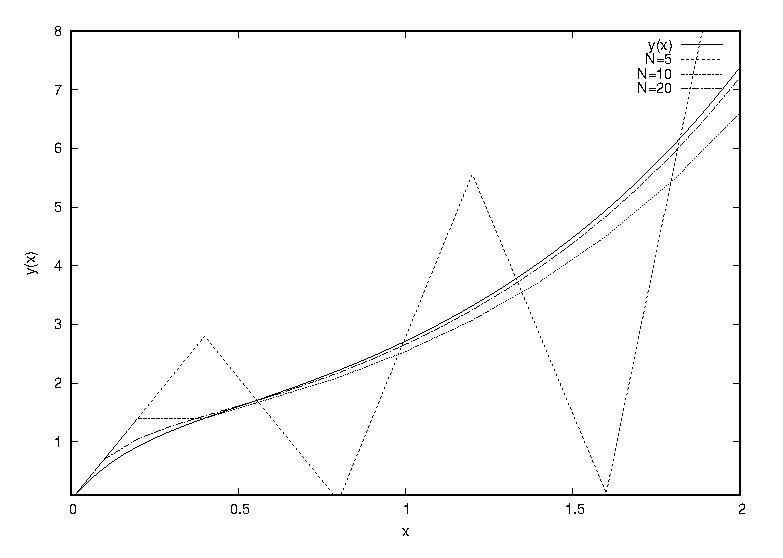
\includegraphics[height=7cm]{2/y(t).eps}
	\caption{y(t)}
	\label{fig:2y(t)}
\end{figure}
また、分割数が$N=20$のとき、求める解は$y\approx 2.66$となる。

\section{考察}
どちらの問題も共通して、分割数を多くすればするほど真の解に近づくが、分割数は20程度でも精度の良い解が
得られることがグラフから分かる。
\end{document}




























